% ============================================================
% MAT670 -- Lecture 1 (source: MAT670_1, pp. 1--17)
% ============================================================
\chapter{Lecture 1: Packing problems}
\label{L1:chap}

\section{Course format}
\label{L1:sec:admin}
\orig{1.0 ``Admin'': contact, room, breaks omitted}
Evaluation is by short quizzes and a project: a talk of at least 20 minutes
together with a written summary. Updates are posted by email, through TU Online,
and on the course page \texttt{wkusner.github.io/MAT670/}.

\section{Mathematics of packings, lattices and configurations}
\label{L1:sec:overview}

The subject of this course sits at the meeting point of several areas:
\begin{itemize}[nosep]
  \item classical convex and discrete geometry, and the geometry of numbers;
  \item applied topology and Morse theory;
  \item statistical mechanics, combinatorics and information theory.
\end{itemize}
\orig{p.\,1: a diagram linking these areas; ``Rigidity'' crossed out there}
We will take various ideas from each of these, all of them dealing with
\emph{configurations} of points or bodies. Related topics include rigidity theory
and configuration spaces of linkages, information theory (codes), and the geometry
of numbers. Packing problems are my main motivation.

Packing problems are typically \emph{easy to state but hard to solve}. The same
is true of the geometric inequalities and the configuration spaces we will meet
along the way.

\begin{remark}
\added{Some landmarks, for orientation: the densest packing of congruent balls
in $\R^3$ (the Kepler conjecture, density $\pi/\sqrt{18}$) was proved by Hales
(announced 1998, published 2005; formal verification by the Flyspeck project 2014/2017).
In dimension $8$ the $E_8$ lattice packing was proved optimal by Viazovska (2016),
and in dimension $24$ the Leech lattice packing by
Cohn--Kumar--Miller--Radchenko--Viazovska (2016/2017). These dimension $8$ and $24$
results appeared during the course itself. In every other dimension
$d\ge 4$ the problem is still open.}
\end{remark}

\section{Packing problems}
\label{L1:sec:packing}

\subsection{Packing congruent bodies in a box}

We start in two dimensions, with the problem of packing circles (disks) in a box.
Let $B\subset\R^2$ be a box (a square, say) and $K$ a disk. We want to place $N$
congruent copies of $K$ in $B$ so as to maximize the \emph{density}, or volume fraction,
\[
  \frac{\vol\bigl(\bigcup_{i=1}^N K_i\bigr)}{\vol(B)} .
\]

\begin{center}
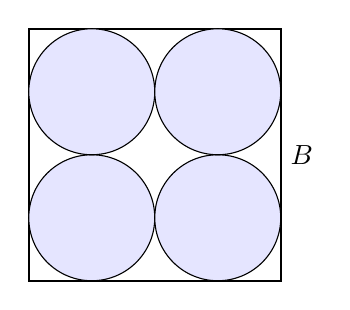
\begin{tikzpicture}[scale=0.8]
  \draw[thick] (0,0) rectangle (4,4);
  \foreach \x/\y in {1/1,3/1,1/3,3/3} \draw[fill=blue!10] (\x,\y) circle (1);
  \node[right] at (4,2) {$B$};
\end{tikzpicture}
\\[2pt]
{\small \added{Four congruent disks packed in a square $B$ (this $2\times2$ arrangement is optimal for $N=4$).}}
\end{center}

\begin{definition}[Packing in a box]
\label{L1:def:packing-box}
A collection $K_1,\dots,K_N$ of subsets of $\R^n$ is a \emph{packing of $K$ in $B$} if
\begin{enumerate}[nosep]
  \item the $K_i$ are congruent to $K$: $K_i=\varphi_i K$ with
        $\varphi_i\in\R^n\rtimes\SO(n)$ a rigid motion\added{;}
  \item $K_i\subset B$ for all $i$\added{;}
  \item the interiors are pairwise disjoint: $\interior K_i\cap\interior K_j=\emptyset$
        for $i\neq j$.
\end{enumerate}
\end{definition}
\orig{p.\,3 writes $\R^2\rtimes\SO(2)$}

\begin{example}
\label{L1:ex:radius}
Two equivalent formulations of the disk-in-a-box problem:
\begin{enumerate}[nosep]
  \item Find the largest scale $r$ such that $\bigcup_{i=1}^N \varphi_i(rK)\subset B$ is
        a packing of $B$\added{, where $K$ is the unit disk}. (Here $rK$ is in Minkowski notation:
        $rK=\{rx : x\in K\}$.)
  \item Find a configuration $\{x_1,\dots,x_N\}$ of $N$ points in $B$ such that
        \[
          d(x_i,x_j)\ \ge\ 2r \quad\text{for } i\ne j,
          \qquad\text{and}\qquad d(x_i,\partial B)\ \ge\ r \quad\text{for all } i,
        \]
        with $r$ as large as possible.
\end{enumerate}
\fixed{notes: $d(x_i,x_j)>r$; disks of radius $r$ need centres $2r$ apart}
\added{The points $x_i$ are the centres of the disks $\varphi_i(rK)$.}
\end{example}

These are hard problems, and there is an infinite variety of them: we can change
$N$, $K$ and $B$, the dimension, add other constraints, and so on.

One case of particular interest is $B=\R^2$: the circle packing problem in the
plane. Other natural choices are $B=\R^d$, or $B=\Sph^2$.
\added{(For $B=\R^d$ the number of bodies is infinite and ``density'' must be
defined by a limit; this is done next.)}

\subsection{Packings of the plane}
\label{L1:subsec:plane}
\orig{numbered ``1.2'' a second time in the notes}

Now take $B=\R^2$. We have an infinite collection of congruent disks $K_i$, now
normalized to have unit radius, with $\interior K_i\cap\interior K_j=\emptyset$ for $i\ne j$.
Write $P=\bigcup_i K_i$.

\begin{definition}[Upper and lower density]
\label{L1:def:density}
The \emph{upper density} of the packing $P$ is
\[
  \dens^+(P)\;=\;\limsup_{R\to\infty}\frac{\vol(P\cap R\,\mathbb{D}^2)}{\vol(R\,\mathbb{D}^2)},
\]
where $\mathbb{D}^2$ is the closed unit disk \added{centred at the origin}.
The \emph{lower density} $\dens^-(P)$ is defined in the same way with $\liminf$.
In general dimension,
\[
  \dens^+(P)\;=\;\limsup_{R\to\infty}\frac{\vol(P\cap R\,\mathbb{D}^n)}{\vol(R\,\mathbb{D}^n)}
\]
\added{with $\mathbb{D}^n$ the unit ball in $\R^n$}.
\end{definition}

\begin{remark}
These quantities need not be nice in general \added{(e.g.\ $\dens^+(P)\neq\dens^-(P)$
is possible, and then ``the'' density of $P$ is not defined)}. However:
\begin{itemize}[nosep]
  \item they do \emph{not} depend on the choice of origin \added{(moving the centre
        changes the numerator only in a boundary layer of volume $O(R^{n-1})$)};
  \item they \emph{do} depend, in general, on the shape of the averaging region
        $\mathbb{D}^n$ \added{(for periodic packings, though, any reasonable shape gives the same value)}.
\end{itemize}
\end{remark}

Does a packing of maximal density exist? We might look at this in more detail later.
\added{(It does: the supremum of $\dens^+$ over all packings is attained, by a compactness
argument; see e.g.\ Groemer's theorem in Conway--Sloane, \emph{Sphere Packings, Lattices
and Groups}, Ch.~1.)}
\unclear{existence deferred in the notes}

\subsection{Bounds on the density}

How can we compute bounds on the density? Clearly $\dens^+(P)\le 1$, which is a bad bound.

We can also construct lower bounds using highly structured packings. For example,
the unit balls centred at the points of $(2\Z)^d$ form a packing. Since this structure
is periodic, we can work with the fundamental domain.

\begin{exercise}[Easy]
\label{L1:ex:periodic-density}
Why can we compute the density on a fundamental domain? \added{Show that for a periodic
packing, with period lattice $\Lat$ and $m$ balls of radius $1$ centred in a fundamental
domain $F$ of $\Lat$, the density exists (that is, $\dens^+=\dens^-$) and equals
$m\,\vol(\Ball^d)/\vol(F)$.}
\end{exercise}

Recall the volume of the ball of radius $r$ in $\R^d$:
\[
  V_d(r)\;=\;\vol\bigl(\Ball^d(r)\bigr)\;=\;\frac{\pi^{d/2}}{\Gamma\!\left(\frac d2+1\right)}\,r^d .
\]
This is easier to remember in even dimension: $V_{2k}(r)=\dfrac{\pi^k}{k!}\,r^{2k}$.
For $(2\Z)^d$ the fundamental domain is the cube $[0,2)^d$ of volume $2^d$, containing one
ball, so the density is
\[
  \dens\bigl((2\Z)^d\bigr)\;=\;\frac{V_d(1)}{2^d}\;=\;\frac{\pi^{d/2}}{\Gamma\!\left(\frac d2+1\right)2^d}
  \;\overset{d=2k}{=}\;\frac{\pi^{k}}{k!\,2^{2k}} .
\]
\orig{notes write $(\tfrac d2)!$ for $\Gamma(\tfrac d2+1)$}

We could improve this by considering better periodic systems.

\begin{exercise}[Easy]
\label{L1:ex:periodic-approx}
Show that periodic packings can approximate a densest packing: \added{the supremum of
$\dens^+(P)$ over all packings $P$ equals the supremum over periodic packings.
(Hint: cut a large cube out of a near-optimal packing, remove the balls that meet its
boundary, and repeat periodically.)}
\end{exercise}

But which periodic systems should we use?

\begin{exercise}
\label{L1:ex:root-lattices}
Consider the lattices coming from the root systems $A_1\times\cdots\times A_1$
($d$ factors), \dots, $A_d$. Compute their packing densities and compare.
\unclear{p.\,6: ``Consider $A^1$, $A_1\times^d A_1$ \dots\ $A_d$? root systems''}
\added{(For reference: $A_1^d$ gives $\Z^d$, which is $(2\Z)^d$ after scaling, with
density $V_d(1)/2^d$. The lattice $A_d$ has minimal norm $\sqrt2$ and covolume
$\sqrt{d+1}$, hence density $V_d(1)\,2^{-d/2}/\sqrt{d+1}$. This gives
$\pi/\sqrt{12}$ for $d=2$ and $\pi/\sqrt{18}$ (FCC) for $d=3$.)}
\end{exercise}

\section{A better bound (non-constructive)}
\label{L1:sec:saturation}
\orig{\S1.3 in the notes}

\begin{definition}[Saturated packing]
\label{L1:def:saturated}
A packing $P=\bigcup_i K_i$ of congruent copies of $K$ in $\R^n$ is \emph{saturated} if
$P\cup\varphi K$ is not a packing for any $\varphi\in\R^n\rtimes\SO(n)$; that is,
no additional disk (ball) can be added.
\end{definition}

\begin{itemize}[nosep]
  \item Saturated packings certainly exist: \added{start from any packing and keep adding
        balls}. This is an ``infinite algorithm''. \added{It can be made rigorous with
        Zorn's lemma, or by adding balls greedily along an enumeration of a countable
        dense set of centres.}
  \item Saturation does not decrease $\dens^+(P)$ \added{since we only add balls}.
\end{itemize}
So for lower bounds on the best possible density we may assume that $P$ is saturated.

This is a surprisingly useful idea. Let $K$ be the unit ball, $K_i=\varphi_i K$ with centre $c_i$.

\begin{proposition}
\label{L1:prop:saturated-bound}
If $P$ is a saturated packing of unit balls in $\R^d$, then $\dens^+(P)\ge 2^{-d}$.
\end{proposition}

\begin{proof}
If $P$ is saturated, then for every $x\in\R^d$ there is an $i$ with $d(x,K_i)<1$.
\added{Otherwise $|x-c_i|\ge 2$ for all $i$, and the unit ball centred at $x$ could be added.}
Hence the doubled balls
\[
  2K_i\;:=\;\varphi_i\bigl(2\,\varphi_i^{-1}(K_i)\bigr)\;=\;\Ball(c_i,2)
\]
form a covering of $\R^d$. \added{Each $2K_i$ has $2^d$ times the volume of $K_i$, so the
fraction of $R\,\mathbb{D}^d$ covered by $\bigcup_i 2K_i$ is, up to a boundary term that
vanishes as $R\to\infty$, at most $2^d$ times the fraction covered by $P$. Since the
doubled balls cover everything,}
\[
  2^d\,\dens^+(P)\ \ge\ 1,\qquad\text{i.e.}\qquad \dens^+(P)\ \ge\ \frac1{2^d}. \qedhere
\]
\end{proof}
\orig{boxed correction: dilate about the centre, $(2\varphi_i^{-1}K)\varphi_i$}

\begin{remark}
\added{Compare with $(2\Z)^d$, of density $V_d(1)/2^d$. Since $V_d(1)<1$ exactly for
$d\ge13$, and $V_d(1)\to0$ superexponentially, the non-constructive bound $2^{-d}$ is
the better one in high dimensions.}
\end{remark}

We may go over some slight improvements in the future, but none seem satisfying.
\begin{remark}
\added{Known improvements of the $2^{-d}$ lower bound include the bound of
Minkowski and Hlawka
($2\zeta(d)\,2^{-d}$), Rogers and Ball ($c\,d\,2^{-d}$), Venkatesh 2013
($c\,d\log\log d\,2^{-d}$ along a sparse sequence of $d$), and, after the course,
Campos, Jenssen, Michelen and Sahasrabudhe 2023 ($c\,d\log d\,2^{-d}$) and
Klartag 2025 ($c\,d^2\,2^{-d}$). All of them are only polynomial improvements over $2^{-d}$.}
\end{remark}

The problem is that there is much more freedom in dimensions $d>3$!
\unclear{``$d>3$! even.'': perhaps ``even $d=4$''}
For example, take $(2\Z)^4$. The main diagonal of the cube $[0,2]^4$ has length
$2\sqrt4=4$, so the centre $(1,1,1,1)$ is at distance $2$ from every vertex.
\added{So a unit ball fits into every such hole. Adding them gives the
$D_4$ packing $(2\Z)^4\cup\bigl((2\Z)^4+(1,1,1,1)\bigr)$, which has twice the density,
$\pi^2/16$.}

\section{Upper bounds in dimension 2}
\label{L1:sec:upper2}
\orig{\S1.4}

The lower bound in $d=2$ is constructive: it comes from the hexagonal (triangular) lattice packing.

\begin{center}
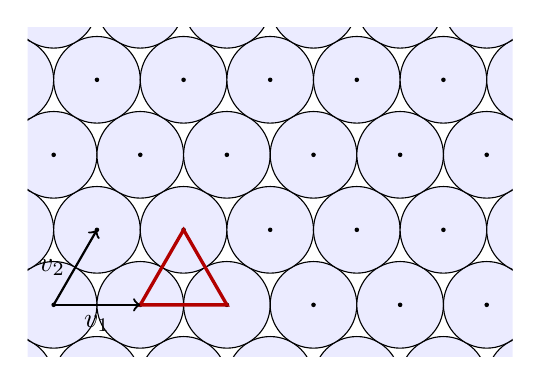
\begin{tikzpicture}[scale=0.55]
  \clip (-0.6,-1.2) rectangle (10.6,6.4);
  \foreach \j in {-1,0,1,2,3,4} {
    \foreach \i in {-3,...,6} {
      \pgfmathsetmacro{\x}{2*\i+\j}
      \pgfmathsetmacro{\y}{sqrt(3)*\j}
      \draw[fill=blue!8] (\x,\y) circle (1);
      \fill (\x,\y) circle (1.5pt);
    }
  }
  \draw[very thick,red!70!black] (2,0) -- (4,0) -- (3,{sqrt(3)}) -- cycle;
  \draw[->,thick] (0,0) -- (2,0) node[midway,below] {$v_1$};
  \draw[->,thick] (0,0) -- (1,{sqrt(3)}) node[midway,left] {$v_2$};
\end{tikzpicture}
\\[2pt]
{\small Hexagonal packing of unit disks, basis $v_1=(2,0)$, $v_2=(1,\sqrt3)$ \added{(angle $\pi/3$)}, and an equilateral triangle of side $2$.}
\end{center}

\begin{example}[Hexagonal packing]
\label{L1:ex:hex}
Consider the equilateral triangle of side $2$ spanned by three mutually tangent unit disks.
Its height is $\sqrt{2^2-1^2}=\sqrt3$, so its area is $\sqrt3$. It contains three
sectors of angle $\pi/3$, i.e.\ half a unit disk, of area $\pi/2$. The plane is tiled by
such triangles, so
\[
  \dens_{\mathrm{hex}}\;=\;\frac{\pi/2}{\sqrt3}\;=\;\frac{\pi}{2\sqrt3}\;=\;\frac{\pi}{\sqrt{12}}\;\approx\;0.9069 .
\]
\end{example}

\subsection{Lattice packings}

For lattices, we want to maximize the minimum distance between two points of a unit lattice
\added{(a lattice $\Lat\subset\R^2$ of covolume $1$)}.
\orig{crossed out: ``minimize the det of the span for a unit lattice''}
This minimum distance can be arbitrarily small, but it is bounded above.

\begin{theorem}[\added{Lagrange}]
\label{L1:thm:lattice2}
Every lattice packing of congruent disks in $\R^2$ has density at most $\pi/\sqrt{12}$.
\added{Equality holds only for the hexagonal lattice.}
\end{theorem}

\begin{proof}
Scale so that $\Lat$ has covolume $1$, and let $2r$ be its minimal distance, so that disks of
radius $r$ centred at $\Lat$ form a packing of density $\pi r^2$. Let $v$ be a shortest
vector, $|v|=2r$. The lattice is the union of translates of the row $\Z v$, which lie on
parallel lines. Since the covolume is $1$, adjacent lines are at distance $h=1/(2r)$.
Note that this is the height of a fundamental parallelogram; the second basis vector
need not be orthogonal to $v$.

\begin{center}
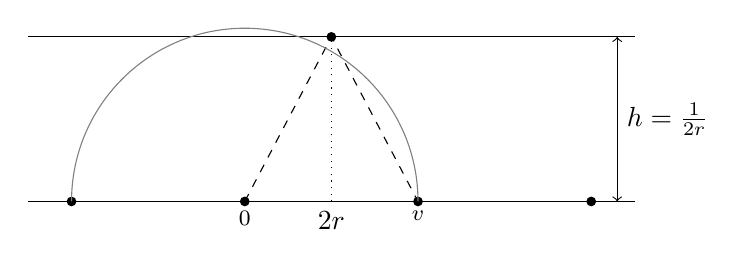
\begin{tikzpicture}[scale=1.1]
  \draw (-0.5,0) -- (6.5,0);
  \draw (-0.5,1.9) -- (6.5,1.9);
  \foreach \x in {0,2,4,6} \fill (\x,0) circle (1.6pt);
  \fill (3,1.9) circle (1.6pt);
  \draw[dashed] (2,0) -- (3,1.9) -- (4,0);
  \draw[dotted] (3,0) -- (3,1.9);
  \draw[gray] (2,0) ++(0:2) arc (0:180:2);
  \node[below] at (3,0) {$2r$};
  \draw[<->] (6.3,0) -- (6.3,1.9) node[midway,right] {$h=\frac1{2r}$};
  \node[below] at (2,0) {\footnotesize $0$};
  \node[below] at (4,0) {\footnotesize $v$};
\end{tikzpicture}
\end{center}

\added{Translating along the row by multiples of $v$, we may take a lattice point $w$ in the
adjacent row whose orthogonal projection onto the first line lies within distance $r$ of
some lattice point there.} Since $|w-u|\ge 2r$ for all lattice points $u\ne w$,
\[
  h^2+r^2\;\ge\;(2r)^2,\qquad\text{so}\qquad \frac1{2r}\;=\;h\;\ge\;\frac{\sqrt3}{2}\,(2r)\;=\;\sqrt3\,r .
\]
Hence $r^2\le \frac1{2\sqrt3}$, i.e.\ $2r\le\sqrt{2/\sqrt3}$, and
\[
  \dens\;=\;\frac{\pi r^2}{1}\;\le\;\frac{\pi}{2\sqrt3}\;=\;\frac{\pi}{\sqrt{12}} .
\]
\added{Equality forces $h=\sqrt3 r$ with offset exactly $r$, which is the hexagonal lattice.}
\end{proof}
\orig{p.\,9 is an unnumbered duplicate of this computation}

\section{Partitioning space: Voronoi cells and Delaunay triangulations}
\label{L1:sec:voronoi}
\orig{\S1.5}

For packings that are not lattices, we need some analogous method to partition space.
Classically, Dirichlet--Voronoi diagrams work well.

\begin{definition}[Voronoi cell]
\label{L1:def:voronoi}
Given a packing with bodies $P_i$, the \emph{(Dirichlet--)Voronoi cell} associated with $P_i$ is
\[
  D_i\;=\;\{x\in\R^2 : d(x,P_i)<d(x,P_j)\ \text{for all } j\neq i\}.
\]
\end{definition}

When the $P_i$ are congruent disks and $d$ is the standard distance, this is the same as using
the distance to the centres of the disks. \added{Indeed $d(x,P_i)=|x-c_i|-1$ for $x\notin P_i$.}

Voronoi cells have nice properties:
\begin{itemize}[nosep]
  \item each cell is an intersection of half-spaces determined by the centres
        \added{($D_i=\bigcap_{j\ne i}\{x:|x-c_i|<|x-c_j|\}$)}, so it is convex;
  \item the cells partition space up to a boundary term \added{(a set of measure zero)}.
\end{itemize}

\begin{center}
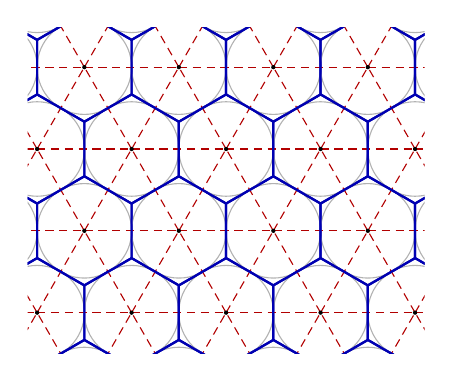
\begin{tikzpicture}[scale=0.6]
  \clip (-3.2,-2.6) rectangle (5.2,4.3);
  \foreach \j in {-2,...,3} {
    \foreach \i in {-3,...,4} {
      \pgfmathsetmacro{\x}{2*\i+\j}
      \pgfmathsetmacro{\y}{sqrt(3)*\j}
      \draw[gray!60] (\x,\y) circle (1);
      \draw[blue!70!black,thick] (\x,\y) ++(30:1.1547) -- ++(150:1.1547) -- ++(210:1.1547)
         -- ++(270:1.1547) -- ++(330:1.1547) -- ++(30:1.1547) -- cycle;
      \draw[red!70!black,densely dashed] (\x,\y) -- ++(2,0);
      \draw[red!70!black,densely dashed] (\x,\y) -- ++(1,{sqrt(3)});
      \draw[red!70!black,densely dashed] (\x,\y) -- ++(-1,{sqrt(3)});
      \fill (\x,\y) circle (1.3pt);
    }
  }
\end{tikzpicture}
\\[2pt]
{\small \added{Hexagonal packing: Voronoi cells (solid hexagons) and Delaunay triangles (dashed).}}
\end{center}

The dual notion is the \emph{Delaunay triangulation}.
\begin{itemize}[nosep]
  \item It is not unique in general (e.g.\ four points at the vertices of a square).
  \item It is harder to define directly. Its characterization: the circumcircles of the
        Delaunay triangles are empty of other points (vertices).
  \item The circumcentre of a Delaunay triangle is a Voronoi vertex.
\end{itemize}
\begin{addedblock}
Precisely: for a locally finite set $X\subset\R^2$ (here, the centres), a triangle with vertices
in $X$ is \emph{Delaunay} if its open circumdisk contains no point of $X$. A Delaunay triangulation is
a triangulation of (the convex hull of) $X$ by Delaunay triangles. It is unique when no four
points of $X$ are concyclic.
\end{addedblock}

\subsection{Existence via lifting}

Consider a collection of points in the plane and lift them to the paraboloid
$z=x^2+y^2$.

\begin{lemma}
\label{L1:lem:lifting}
Let $a,b,c,d$ be points in the $(x,y)$-plane, and lift them to
$\hat a,\hat b,\hat c,\hat d$ on $z=x^2+y^2$ \added{(i.e.\ $\hat p=(p,|p|^2)$)}. Then $d$ lies
inside the circumcircle of $a,b,c$ if and only if $\hat d$ lies in the lower half-space of the
plane $\langle\hat a,\hat b,\hat c\rangle$ \added{spanned by $\hat a,\hat b,\hat c$}.
\end{lemma}

\begin{proof}
A plane tangent to the paraboloid at the point above $(p,q)$ has the form
\[
  z\;=\;2px+2qy-(p^2+q^2).
\]
Shifting it up by $h^2$ gives
\[
  z\;=\;2px+2qy-(p^2+q^2)+h^2 .
\]
\fixed{signs: notes have $+(p^2+q^2)$ and $(x+p)^2$, $(y+q)^2$}
It meets the paraboloid where
\[
  x^2+y^2\;=\;2px+2qy-(p^2+q^2)+h^2
  \quad\Longleftrightarrow\quad (x-p)^2+(y-q)^2\;=\;h^2 .
\]
So the plane through $(p,q,p^2+q^2)$, parallel to the tangent plane there, at height $h^2$
above it, projects its intersection with the paraboloid onto the circle of radius $h$
about $(p,q)$ in the $(x,y)$-plane.
\begin{addedblock}
Every non-vertical plane $z=\alpha x+\beta y+\gamma$ meeting the paraboloid in more than one point
is of this form, with $p=\alpha/2$, $q=\beta/2$ and $h^2=\gamma+p^2+q^2>0$. Apply this to the plane
through $\hat a,\hat b,\hat c$. The corresponding circle passes through $a,b,c$, so it is their
circumcircle. A point $\hat x$ of the paraboloid lies strictly below this plane iff
$x^2+y^2<2px+2qy-(p^2+q^2)+h^2$, i.e.\ iff $(x-p)^2+(y-q)^2<h^2$, i.e.\ iff $x$ lies strictly
inside the circumcircle.
\end{addedblock}
\end{proof}

\begin{corollary}[Existence of Delaunay triangulations]
\label{L1:cor:delaunay-exists}
The existence of the convex hull of the lifted points implies the existence of a Delaunay triangulation.
\added{More precisely: project the faces of the lower convex hull of $\{\hat x:x\in X\}$ to the plane.
By Lemma~\ref{L1:lem:lifting}, a lower face has no lifted point below its plane, so its projection has
an empty circumcircle. Triangulating any non-triangular faces (which come from concyclic points)
gives a Delaunay triangulation. For the infinite, locally finite point sets of a packing, apply this
to large finite pieces; the triangles near a fixed point stabilize.}
\end{corollary}

\section{Thue's theorem}
\label{L1:sec:thue}
\orig{\S1.6; a first ``1.6 Thm'' on p.\,13 is abandoned}

Let $P$ be a saturated packing of unit disks in $\R^2$ and $DT$ a Delaunay triangulation of its set of
centres. Every edge of $DT$ has length at least $2$, since the disks do not overlap.
\added{Moreover, every triangle of $DT$ has circumradius $R<2$. Its open circumdisk contains no
centres, so the circumcentre is at distance $\ge R$ from every centre. If $R\ge2$, a unit disk centred
there could be added, contradicting saturation.}

\begin{lemma}
\label{L1:lem:angle}
The largest angle $\theta$ of a triangle $ABC\in DT$ of a saturated packing satisfies
\[
  \frac\pi3\;\le\;\theta\;<\;\frac{2\pi}3 .
\]
\end{lemma}
\unclear{upper inequality written ambiguously; the proof gives strict ``$<$''}

\begin{proof}
The lower bound is obvious, since $\theta$ is the largest angle of a triangle.
Assume $\theta\ge 2\pi/3$. Let $A$ be the smallest angle. Then $A\le\frac12(\pi-\theta)\le\pi/6$,
so $\sin A\le\frac12$. By the circumradius formula, and since the side $BC$ opposite $A$ has
length at least $2$,
\[
  R\;=\;\frac12\,\frac{|BC|}{\sin A}\;\ge\;\frac12\cdot\frac{2}{1/2}\;=\;2 .
\]
\fixed{notes: ``$=4$''; $\frac12\cdot\frac{2}{1/2}=2$}
\added{This contradicts $R<2$.}
\end{proof}

\begin{lemma}
\label{L1:lem:triangle-density}
The density in a single Delaunay triangle is at most $\pi/\sqrt{12}$, with equality
if and only if the triangle is equilateral \added{(of side $2$)}.
\end{lemma}
\begin{addedblock}
Here the \emph{density} of a triangle $T\in DT$ means $\frac{\pi/2}{\operatorname{area}(T)}$:
the three sectors of the unit disks at the vertices of $T$ have angles summing to $\pi$, hence total area $\pi/2$.
\end{addedblock}

\begin{proof}
Let $B$ be the largest angle of $ABC$. Then
\[
  \operatorname{area}(ABC)\;=\;\tfrac12\,|AB|\,|CB|\,\sin B
  \;\ge\;\tfrac12\cdot2\cdot2\cdot\min_{B\in[\pi/3,\,2\pi/3)}\sin B
  \;=\;\tfrac12\cdot2\cdot2\cdot\tfrac{\sqrt3}{2}\;=\;\sqrt3,
\]
using Lemma~\ref{L1:lem:angle}, and the minimum is attained at $B=\pi/3$. So $\operatorname{area}(T)\ge\sqrt3$
for every $T\in DT$, and the density of $T$ is at most $\frac{\pi/2}{\sqrt3}=\frac{\pi}{2\sqrt3}=\frac{\pi}{\sqrt{12}}$.
\added{Equality requires $|AB|=|CB|=2$ and $B=\pi/3$, i.e.\ an equilateral triangle of side $2$.}
\end{proof}

\begin{theorem}[\added{Thue; Fejes T\'oth}]
\label{L1:thm:thue}
Every packing $P$ of unit disks in the plane satisfies $\dens^+(P)\le\pi/\sqrt{12}$.
\end{theorem}

\begin{proof}
\added{Saturating $P$ does not decrease $\dens^+$ (\S\ref{L1:sec:saturation}), so we may assume $P$ is saturated.}
For a finite union of Delaunay triangles, the density is
\[
  \sum_{T\in DT}\frac{\operatorname{area}(T)}{\operatorname{area}(DT)}\cdot\dens(T)
  \;\le\;\frac{\pi}{\sqrt{12}},
\]
a weighted average of the densities of the triangles, each at most $\pi/\sqrt{12}$
by Lemma~\ref{L1:lem:triangle-density}. Hence any finite union of Delaunay triangles has density
at most $\pi/\sqrt{12}$.

For a large disk $R\,\mathbb{D}^2$, most of its area is covered by the Delaunay triangles inside it,
so the error in the limit is a boundary term.
\begin{addedblock}
Every Delaunay triangle has circumradius $<2$, so diameter $<4$. Let $U_R$ be the union of the
triangles meeting $R\,\mathbb{D}^2$. Then $R\,\mathbb{D}^2\subset U_R\subset(R+4)\mathbb{D}^2$. The sectors
in the triangles of $U_R$ account for every disk centred in $R\,\mathbb{D}^2$. The disks meeting
$R\,\mathbb{D}^2$ but centred outside it lie in the annulus $(R+1)\mathbb{D}^2\setminus(R-1)\mathbb{D}^2$, of area $O(R)$. So
\[
  \vol(P\cap R\,\mathbb{D}^2)\;\le\;\frac{\pi}{\sqrt{12}}\,\vol(U_R)+O(R)
  \;\le\;\frac{\pi}{\sqrt{12}}\,\pi(R+4)^2+O(R).
\]
Dividing by $\pi R^2$ and letting $R\to\infty$ gives $\dens^+(P)\le\pi/\sqrt{12}$.
\end{addedblock}
\end{proof}
\orig{p.\,16 sketch: large concentric disks}

\begin{remark}
\added{Combined with Example~\ref{L1:ex:hex}, this shows that the hexagonal packing is the
densest packing of congruent disks in the plane. The statement goes back to Thue (1892, 1910).
The first proof generally accepted as complete is due to L.~Fejes T\'oth (1940); the argument above
follows his Delaunay-triangle approach. For lattice packings the result is Lagrange's
(Theorem~\ref{L1:thm:lattice2}).}
\end{remark}
